\documentclass[aspectratio=169,12pt]{beamer}
\usepackage[utf8]{inputenc}
\usepackage{amsmath, amssymb}
\usepackage{booktabs}
\usepackage{colortbl}
\usepackage{hyperref}
\usepackage{makecell}
\usepackage{ragged2e}
\usepackage{bytefield}
\usepackage{tikz}
\usetikzlibrary{arrows.meta, positioning, shapes.geometric, calc, tikzmark, shapes.misc, fit, backgrounds}
\usepackage{tcolorbox}
\usetheme{Madrid}

\title{Computer Architecture}
\subtitle{Exercise 1: Performance Evaluation Parameters \& Amdahl's Law}
\author{Course 234267}
\date{}

\begin{document}

\frame{\titlepage}

\begin{frame}{Cache Coherence Flow}
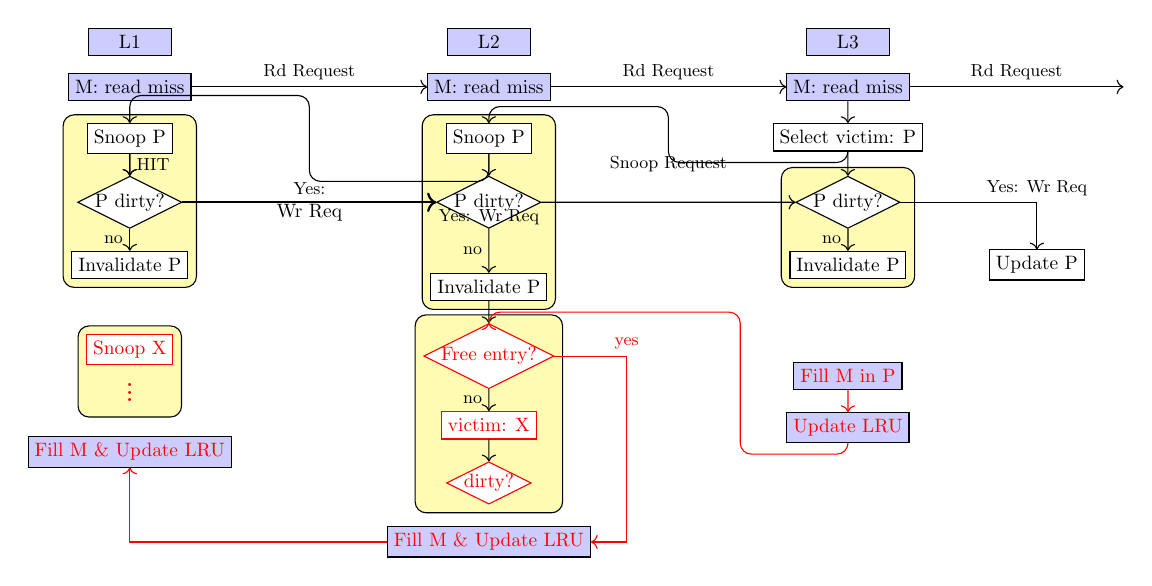
\begin{tikzpicture}[
    scale=0.7, transform shape,
    box/.style={rectangle, draw, minimum width=1.5cm, minimum height=0.5cm},
    decision/.style={diamond, draw, aspect=2, inner sep=0pt, minimum width=1cm, fill=white},
    reddecision/.style={decision, draw=red, text=red},
    bluebox/.style={box, fill=blue!20},
    yellowbox/.style={box, fill=yellow},
    whitebox/.style={box, fill=white},
    redbox/.style={box, fill=white, draw=red, text=red},
    bluered/.style={bluebox, text=red},
    yellowbg/.style={fill=yellow!30, draw=black, rounded corners, inner sep=3pt},
    every edge/.style={draw, ->, >=stealth},
    node distance=0.4cm and 1.5cm
]

% L1 Section
\node[bluebox] (l1) {L1};
\node[bluebox, below=0.3cm of l1] (l1read) {M: read miss};

\node[whitebox, below=of l1read] (snoopp1) {Snoop P};
\node[decision, below=of snoopp1] (dirty1) {P dirty?};
\node[whitebox, below=of dirty1] (inv1) {Invalidate P};
\node[redbox, below=1cm of inv1] (snoopx1) {Snoop X};
\node[below=0cm of snoopx1.south, text=red, anchor=north] (ldotsx1) {\textbf\vdots};

% L2 Section  
\node[bluebox, right=5cm of l1] (l2) {L2};
\node[bluebox, below=0.3cm of l2] (l2read) {M: read miss};

\node[whitebox, below=of l2read] (snoopp2) {Snoop P};
\node[decision, below=of snoopp2] (dirty2) {P dirty?};
\node[whitebox, below=0.8cm of dirty2] (inv2) {Invalidate P};

\node[reddecision, below=of inv2] (free) {Free entry?};
\node[redbox, below=of free] (victimx) {victim: X};
\node[reddecision, below=of victimx] (dirtyx) {dirty?};

% L3 Section
\node[bluebox, right=5cm of l2] (l3) {L3};
\node[bluebox, below=0.3cm of l3] (l3read) {M: read miss};

\node[whitebox, below=of l3read] (select3) {Select victim: P};
\node[decision] at (select3 |- dirty2) (dirty3) {P dirty?};
\node[whitebox, below=of dirty3] (inv3) {Invalidate P};
\node[whitebox, right=of inv3] (update) {Update P};

\node[bluered, below=1.5cm of inv3] (fillm3) {Fill M in P};
\node[bluered, below=of fillm3] (updatelru) {Update LRU};
\node[bluered, below=of dirtyx] (fillm2) {Fill M \& Update LRU};
\node[bluered, below=1.3cm of snoopx1] (fillm1) {Fill M \& Update LRU};

\begin{scope}[on background layer]
\node[yellowbg, fit=(snoopp1)(dirty1)(inv1)] {};
\node[yellowbg, fit=(snoopx1)(ldotsx1)] {};
\node[yellowbg, fit=(snoopp2)(dirty2)(inv2)] {};
\node[yellowbg, fit=(dirty3)(inv3)] {};
\node[yellowbg, fit=(free)(victimx)(dirtyx)] {};
\end{scope}

% Arrows with labels
\draw[->] (l1read) -- node[above, sloped] {\small Rd Request} (l2read);
\draw[->] (l2read) -- node[above, sloped] {\small Rd Request} (l3read);
\draw[->] (l3read) -- node[above, sloped] {\small Rd Request} ++(5,0);

\draw[->] (snoopp1) -- (dirty1);
\draw[->] (dirty1) -- node[left] {\small no} (inv1);
\draw[thick, ->] (dirty1) -- (dirty2.west) node[midway,align=center] {\small Yes:\\Wr Req};
\draw[->] (snoopp1) -- (dirty1) node[midway, right] {\small HIT};

\draw[->] (snoopp2) -- (dirty2);

% the routed path
\draw[->, rounded corners]
  (snoopp2.south)
  -- ++(0,-0.5)                               % down 0.5
  -| ($(snoopp1)!0.5!(snoopp2)$)                                  % over to midpoint x
  |- ($ (snoopp1.north) + (0,0.5) $)          % up to 0.5 above snoopp1.north
  -- (snoopp1.north);                         % straight down

\draw[->] (dirty2) -- node[left] {\small no} (inv2);

\draw[->](dirty2) node[below, align=center] {\small Yes: Wr Req} -- (dirty3.west);

\draw[->] (inv2) -- (free);
\draw[->, red] (free) -| node[above] {\small yes} ++(2.5,0) |- (fillm2);
\draw[->] (free) -- node[left] {\small no} (victimx);
\draw[->] (victimx) -- (dirtyx);

\draw[->] (l3read) -- (select3);

\draw[->, rounded corners]
  (select3.south)
  -- ++(0,-0.2)                               % down 0.5
  -| ($(snoopp2)!0.5!(select3)$)                                  % over to midpoint x
  node[midway, below, near end, align=center] {\small Snoop Request}
  |- ($ (snoopp2.north) + (0,0.3) $)          % up to 0.5 above snoopp1.north
  -- (snoopp2.north);                         % straight down


\draw[->] (select3) -- (dirty3);
\draw[->] (dirty3) -- node[left] {\small no} (inv3);
\draw[->] (dirty3) -| node[above,midway] {\small Yes: Wr Req} (update);
%\draw[->] (dirty3) -- (wrreq);
%\draw[->] (wrreq) -- node[above] {\small Yes: Wr Req} ++(-1,0);

% Bottom connections
%\draw[red, ->] (dirtyx) edge[bend right=40] node[below] {\small Fill M \& Update LRU} (snoopx1);
%\draw[red, ->] (snoopx1) -- node[left] {\small Snoop + Fill M \& Update LRU} ++(-1.5,0);
%\draw[red, ->] (victimx) edge[bend left] node[right] {\small Fill Data} ++(2.5,-1);
%\draw[red, ->] (free) edge[bend right] node[below] {\small Fill M in P + Update LRU} ++(-2.5,0);

\draw[->, red] (fillm3) -- (updatelru);
\draw[->, red, rounded corners]
  (updatelru.south)
  -- ++(0,-0.2)                               % down 0.5
  -| ($(updatelru)!0.3!(free)$)                                  % over to midpoint x
  |- ($ (free.north) + (0,0.2) $)          % up to 0.5 above snoopp1.north
  -- (free.north);                         % straight down                    % straight down

\draw[->, red] (fillm2) -| (fillm1);

\end{tikzpicture}
\end{frame}

\end{document}